\chapter{Concept}\label{sec:concept}

    % \begin{blockquote}
    %     \paragraph{Intent:} General reminder and answer of RQ's
        
    %     Structure:
    %     \begin{description}
    %         \item[1. Surrogates models combinations] Surrogate model is not universal. Domain-specific $\rightarrow$ Surrogate model portfolio 
    %             \begin{enumerate}
    %                 \item Surrogate model is not universal. Domain-specific $\rightarrow$ \textbf{Surrogate model portfolio}
    %                 \item Objectives have different complexity surface $\rightarrow$ Surrogate model is not universal $\rightarrow$ Describe objectives independently. \textbf{Heterogeneous/Composition surrogate model} 
    %             \end{enumerate}
                  
    %         \item[2. Dynamic sampling plan] Use sampling plan while surrogate is not valid
    %             \begin{enumerate}
    %                 \item Surrogate Validation. Stages and thresholds
    %                 \item Metrics
    %             \end{enumerate}

    %         \item[3. Scalability] Compositional surrogates in many-objective space
    %             \begin{enumerate}
    %                 \item Problem: Random solver on high dimensional space $\rightarrow$ Solution: Light surrogates 
    %                 \item Solving problem in subset of dimensions
    %                 \item Categorical parameters*
    %             \end{enumerate}

    %         \item[4. Discussion] General Conclusions. Infill criteria for Pareto-optimal solutions
    %     \end{description}
    % \end{blockquote}

    \epigraph{``All models are wrong but some are useful``}{\textit{– George Box}}

    This section presented a general idea of a improvement in the surrogate-based optimization for black-box function. 

    The usual optimization problem is a trade-off in producing the best possible multi-objective solution with less effort. Because we consider expensive function, an optimization effort, first of all, means evaluation budget. Each of these evaluations can require much time, energy, or other resources. That is why the main multi-objective comparison criteria are convergence to the Pareto frontier with a limited evaluation budget. It also takes into account the ratio of non-dominant solutions to the total number of measured configurations and their distribution on the Pareto frontier. In this thesis, under solving a multi-objective problem, we intend to find a set of none-dominated points that cover a wide range of objectives values and close as possible to the real Pareto front. If evaluations of the problem are expensive, the real count of experiments could be reduced throw applying a multi-objective algorithm on a surrogate model. This technique is the preferred choice for functional optimization when the evaluation cost is high.

    While multiple algorithms could be applied, we selected \gls{moea} as default optimization techniques for the surrogate models. The advantage of \gls{ea} is that it could be easily modified and it could operate on a set of solutions candidates, that are well-fitted to approximate the Pareto-front. Finally, evolutionary algorithms can estimate highly complex problems in various use-cases.


    %? The main objective of this part is to provide a thorough treatment of multi-objective parameter tuning with evolutionary algorithm(s)


    % The solution techniques and parametric selections however are usually problem-specific. \cite{abs181207958}
    % --------------------------------------------------------------------------------------------
    % ------------------------------------------------     RG1: Models combinations     
    % --------------------------------------------------------------------------------------------

    \section{Surrogates models combinations [RQ1]}

        Let us address the main issue we have observed in multi-objective optimization. Base on the statement that the surrogate model is domain-specific, the central idea of the thesis is introduced as the model variability \emph{in} a surrogate model and the extensibility \emph{with} surrogate hypotheses.

        % ------------------------------------------------     Compositional model       
        \subsection{Compositional Surrogate Model}
            The concept of the compositional surrogate means a combination of the multiple simple models that simulate the several objectives independently at the same time. Dividing optimization problems to several parts improves the variability of surrogates and accordingly, the possibilities to improve the solution.
            Besides, a significant advantage of the compositional surrogate is a possibility to extend the single-objective parameter tuning to the multi-objective task. This provides the opportunity to reuse single-criteria models for multi-criteria optimization and dynamically reconstruct problem representation from mixed parts.
            
            % Nonetheless, the surrogate model is not universal to describe objectives independently. 

            That approach should be capable, outperform static models in adaptation to a real black-box problem with the unknown objective surface. For example, a user could represent his domain knowledge as preferring to a concrete combination of the surrogate models or calibrate it during optimization. 
            
            In this thesis, the \emph{compositional model} means a surrogate model that combines various surrogates models for each optimization objective. The \emph{surrogate hypothesis} refinement is also used to emphasize on the fact that the surrogate model can completely describe all criteria from the objective space.

            % ------------------------------------------------     Scalability     
            \subsubsection{Scalability}
                In practice show that an MOEA is challenging to scale. For many-dimensional problem, more than 10 objectives random solver gain better solution than MOEA. Furthermore, surrogate models also suffer from this. For instance, complexity ob Krigin/Bayesian model increase exponential with growing samples size and dimensionality.
                % ! \todor{examples how to solve it, related work}

                The compositional model could improve the solution by a precisely select group of surrogates to describe problem landscape. Each surrogate model could extrapolate one or subset objectives and together with other model provide a complex hypothesis of how a parameter and objective spaces related.

                As a result, it should allow us to build a useful surrogate model to make a quality many-objective decision in parameter tuning. 

            % -------------------------     Categorical parameters      
            \subsubsection{Categorical parameters} Multi-objectivity and a real/ordinal/categorical parameters are essential for real parameter tuning. There are known two basic approaches to implement this functionality: decision tree or feature encoding and fit arbitrary model. Most related works used native models that support categorical features because it is interpretative and can transform prediction backwards. 
            On the other hand, feature encoding is used to support a categorical parameter for generic models. Coding features for a surrogate model can transform those in a meaningful form, understandable for a surrogate model. Encoding represents a feature in an alternative form that helps model instantiation relation and a correlation between features. Based on this inner interpretation model can predict the values of labels based on a parameter vector. The problem occurs in reverse interpretation of these optimal predictions in the context of parameter space. Often a found solution is not a feasible point from parameters space. As a possible solution, it partly transforms problems in multiple classification tasks and then considers there relation as optimization with continuous probability [TPE]. 
            For the general surrogate model with mixed parameters, we can solve a problem orthogonally with multiple optimizers.  Then general idea consists in sequentially applying several algorithms that use previous results. For example, encode features and fit models as usual. First, apply local search that can evaluate only valid parameters. The solutions found may be satisfactory but not optimal.  The next step is a genetic algorithm that uses the result of the previous algorithm, namely the optimal categories values. The multi-algorithm help achieve the most significant values in the remaining parameters. 

            Such a concept is vital for expensive multi-criterion optimization when the solution space is mixed and has an overwhelming number of real values. 
            
        
        % ------------------------------------------------     Portfolio      
        \subsection{Surrogate model portfolio}
            With gain to find the best solution with less effort surrogate models is domain-specific. It's mean that there is no universal approximation model. It could be interpreter as Non-free lunch theorem in model-based optimization. If we extend this argument, then the same optimization problem with another sample set could be interpreted as another optimization problem. The search space landscape, modality and geometry may hugely differ. The complexity to restore the original problem change during optimization. It depends on how much samples are and which diversity they have.
            This means that to reduce effort and increase the convergence of an algorithm, we should change the surrogate model depend on how much samples do we have. As one would expect, no approximation method is universal. Hence, this leads us to use a portfolio with surrogate models. As a negative consequence, the model fitting introduces an additional overhead into the optimization. 
        
            With the flexibility that provides a compositional system to combine several models, that is valuable to produce several variants of compositions from available surrogates. This functionality requires validation criteria to discard those that are not valid and comparison metrics to range and combine the best ones. There are created many hooks to combine and solve surrogates models. These placeholders give flexibility to the combination of hypotheses, testing, and solving/optimization. Bagging or ensemble technique can be applied to both steps: the surrogate models and the optimization algorithms.

            Besides, it grates motivation to use the latest state-of-the-art algorithms and models together because the modular structure of the compositional model and portfolio allows using it as hooks for optimization.  

    % --------------------------------------------------------------------------------------------
    % ------------------------------------------------     RG2: Sampling plan     
    \section{Sampling plan [RQ2]}
        For expensive optimization problems, it would be useful to modulate a problem using quite a small number of most informative examples. Nonetheless, almost sequential model-based approaches use a static sampling plan. Under the sampling plan may also be assumed randomized designs in design-of-experiment(DOE). If the oracle does not determine the required optimal samples, it can lead to unnecessary waste of valuable evaluation attempts. 
        
        The general idea of how to solve this problem lay on relating initial sampling design to validation the surrogate models. An optimization search is guided by sampling design until that moment when valid surrogate model is presented (Figure \ref{fig:concept_sampling}). Validity means that surrogate approximation could be useful for efficient global optimization.

            % ==== Sampling plan
            \begin{figure}
                \centering
                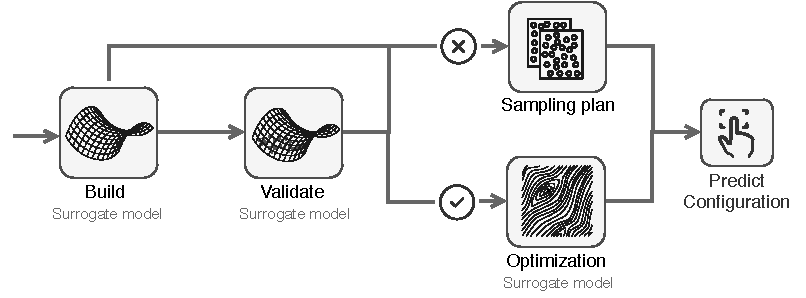
\includegraphics[width=\textwidth]{content/images/dinamic_sampling_plan}
                \caption[Non-dominated points]{Concept of a sampling plan dependency and model validation. A sampling plan is used if there is no valid model that can be useful for optimization purpose.} 
                \label{fig:concept_sampling} 
            \end{figure}      

        % -------------------------     Surrogate Validation      
        \subsection{Surrogate Validation}
        It is necessary to sacrifice a small portion of samples to check the quality of the surrogate model. Based on validation results, we can discard inadequate models and elaborate evaluate the solutions from valid models. If neither model is valid, this means that the best solution right now is a prediction from the sampling plan. This decision is repeated until a valid surrogate model is obtained.
        In the context of sequential model-based optimization, a common misconception lay in prefer global accuracy score over the score in the optimal region. That is why evaluation surrogate validity based only on the coefficient of determination(R2) metrics is incorrect \cite{nardi2019practical}. Global accuracy metric can be used as a threshold value for exceeding which the model becomes not valid even with additional estimations.  

            % ==== train\valid\test
            \begin{figure}
                \centering
                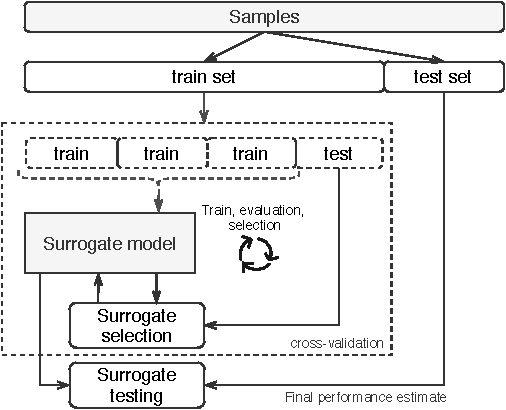
\includegraphics[width=10cm]{content/images/cv}
                \caption[Cross-validation: exploration vs exploitation]{Validation surrogates models. Cross-validation loop performs selection models based on global accuracy; Successful models perform on a test set with a focus on optimization region.} 
                \label{fig:cv}   
            \end{figure}

        The central concept for surrogate validation lay in adaptation best practices from the machine-learning community for evaluation estimator's performance. 

        Validation should show how well the model extrapolates the available experiments and how well it can evaluate the data that is not seen. In the case of validation a several models, results could have not a representative performance if data split only to train/test set.  There is a risk of overfitting on the test data. It means that the test set 'leak' to train set and final metrics does not report on the surrogate achievement. 
        Deal with this problem, yet another portion of samples can handle as a so-called 'validation set.' This new set is used for model selection independently from the test set. When models are selected, final evaluation can be done on the test set. However, partitioning the available samples into three sets, are drastically reduce the number of points which can be used for learning the model. Moreover, results can depend on a selective random decision for the samples splitting.
        
        The solution is might be cross-validation(CV, Figure \ref{fig:cv}). This is a procedure that avoids a separate validation set and divides test samples to \textit{k} equal folds. Set of folds are used to train model and in \textit{k} rounds, a new fold selected as a test set. The performance measure by cross-validation is the average of the values computed in the loop. This approach can be computationally expensive, but requires fewer samples. 
        
        As s result, the concept of a surrogate validation based on two sequential stages:
        \begin{enumerate}
            \item \textbf{Cross-validation.} Evaluate that model performs well to generalize landscape. Select candidates that have enough accuracy.
            \item \textbf{Surrogate testing.} Final evaluation performs on the test set that shows accuracy on the region of interests. In the context of multi-objective optimization, it is non-dominated samples.
        \end{enumerate}
        
        The decision on which surrogate model is better made based on the information from all stages. If the model does not have a sufficient threshold, it is rejected as not valid. If there is no valid model, the assumption of the next configuration is accepted from the sapling plan (Figure \ref{fig:concept_sampling}).

        % overfit - underfit
    
        % metrics comparison


    % --------------------------------------------------------------------------------------------


    % --------------------------------------------------------------------------------------------
    % -----------------------------------------------------       Discussion      ----------------
    \section{Discussion}

        In this thesis, proposed approach for combination surrogates for multi-objective optimization and dynamic sampling plan based on surrogate validation.

        As a reply to RG1 we provide two answers: 1.) Combination complex surrogate model from surrogates on objectives 2.) Comparison of multiple surrogates in the portfolio to select the best one or generate an ensemble of results from all applicable variants.

        % -----------------------------------------------------      Infill criteria       
        \paragraph{}{Infill criteria}
        In the case of MOEA, solution of algorithm present as non-dominated final population. Based on unbiased, multi-objective criteria, they all uniformly could be presented as a prediction to the next evaluation. They represents current solution based on the surrogate model. Nevertheless, there is prior knowledge available in samples which can be taken into account. To reduce the number of candidates in the population, it is possible to deny those in which the distance to the nearest available sample is less than their average distance.
        So there are two strategies for predicting from a population:
        \begin{itemize}
            \item Prior and posterior knowledge. Based on changing metrics in available and proposed solutions
            \item Posterior knowledge. Proposed solutions are all equal
        \end{itemize}


        
        % -----------------------------------------------------       Conclusions       
        Also, to the best of our knowledge, has not been previously or stingy reported in the efficient multi-objective optimization.
        Contribution:
        \begin{itemize}
            \item Surrogate combination/composition with heterogeneous models
                \begin{itemize}
                    \item Surrogate models portfolio
                    \item Compositional surrogate model
                    \item Combination of different(orthogonal) solvers
                \end{itemize}
            \item Surrogate portfolio. Search a better hypothesis  for a specific problem at a particular stage of parameter tuning
            \item Metric combination for evaluation Pareto optimal points
            \item Samples size depends on model(s) validity
            \item Concepts
                \begin{itemize}
                    \item Combination of different(orthogonal) solvers
                    \item Infill criteria for prediction selection
                \end{itemize}
        \end{itemize}

        We argue that the proposed concept from this thesis is the preferred choice for functional optimization when the evaluation cost is large.


        Our work is similar in constitution to the approaches adopted from the expensive MBMO \cite{SoftSurvey} with a modular framework structure that includes a surrogate portfolio. We extend the idea of model selection and k-fold cross-validation to verify how a surrogate(s) model might operate differently on various problem sceneries. To our knowledge, there exists no research that investigates how to make a composition of several surrogate models and use it in a portfolio. Also, there is an open question how this method scales.


        % structures include more than one possibility, as described above. Nevertheless, this level

        % Finally, another aspect worth mentioning is the fact that GSM appears in more than one cell. Indeed, hybrid methods


        % where the algorithms are allowed to query an oracle for additional data to infer better statistical models


        % They also reported that a speedup of a factor of 10 can nevertheless be obtained.



        % With multiple models, their flaws can combine, as well as the time required to build the models. In memetic algorithms, especially if the surrogate model is not very accurate, a local optimum can be found instead of the global optimum. But in terms of parameter tuning, this point should be better than a predefined sampling plan. Evaluation of this prediction improve surrogate model quality in the near-optimal area and improve prediction in the next round.
        % We could describe compositional-based surrogate optimization as compound grey-box system whit a lot of open research areas where surrogate should improve, managing portfolio, compare of predictions Pareto fronts. 
        % As a developer, you can be focused on a specific problem and don't know how to implement other components. This is one of the main advantages of the described approach.

        % less prone to overfitting
        % To our best knowledge, we are the first to make this simple observation, which can be applied to improve any Bayesian hyperparameter
        % optimization method.